\chapter{Levers and Balance Scales}\label{ch:g3:levers-and-scales}

Last year, on the seesaw, we found that weight and distance both
count --- and we promised a precise rule with real numbers in it.
Time to keep the promise. Along the way we will lift stones far too
heavy for our arms, and meet the instrument that weighed the world's
goods for thousands of years.

\section{The lever}

\begin{definition}[Lever and pivot]\label{def:g3:levers-and-scales:lever}
A \emph{lever}\index{lever} is a stiff bar resting on a support
point around which it can tip. The support point is called the
\emph{pivot}\index{pivot}. A seesaw is a lever; so is a crowbar
under a rock, and the claw of a hammer pulling a nail.
\end{definition}

\begin{example}[The strength multiplier]\label{ex:g3:levers-and-scales:crowbar}
A gardener slides a long iron bar under a boulder, rests it on a log
close to the boulder, and presses down on the far end --- and the
boulder, which ten hands could not lift, tips over gently. The
\omterm{def:g3:levers-and-scales:lever}{lever}'s secret is distance: press \emph{far} from the \omterm{def:g3:levers-and-scales:lever}{pivot}, and
your small push does the work of a giant close to it. An old story
says a great scientist of antiquity boasted: ``Give me a place to
stand, and a \omterm{def:g3:levers-and-scales:lever}{lever} long enough, and I shall move the Earth.''
\end{example}

\begin{omfigure}
\begin{tikzpicture}[scale=0.85]
  \draw[thick] (0,0) -- (11,0);
  % fulcrum: flat base on the ground, apex up at (7.6,0.55)
  \draw[thick, fill=omExo, fill opacity=0.3]
    (7.15,0) -- (8.05,0) -- (7.6,0.55) -- cycle;
  % the bar: one straight line resting on the apex and tangent to the
  % rock (computed: through (7.6,0.55), touching the circle at (9.10,0.03))
  \draw[very thick] (1.74,2.57) -- (9.10,0.03);
  % the rock, sitting on the ground, its edge on the bar's tip
  \draw[thick, fill=omExo, fill opacity=0.4] (9.3,0.62) circle (0.62);
  \node[font=\small] at (9.3,0.62) {rock};
  \draw[-Stealth, very thick, omThm] (1.74,3.5) -- (1.74,2.75);
  \node[left, font=\small, omThm] at (1.5,3.15) {small push, far out};
  \node[below, font=\small] at (7.6,-0.3) {pivot close to the rock};
\end{tikzpicture}

{\small The crowbar: a small push far from the \omterm{def:g3:levers-and-scales:lever}{pivot} lifts a heavy
rock close to it.}
\end{omfigure}

\begin{omfigure}
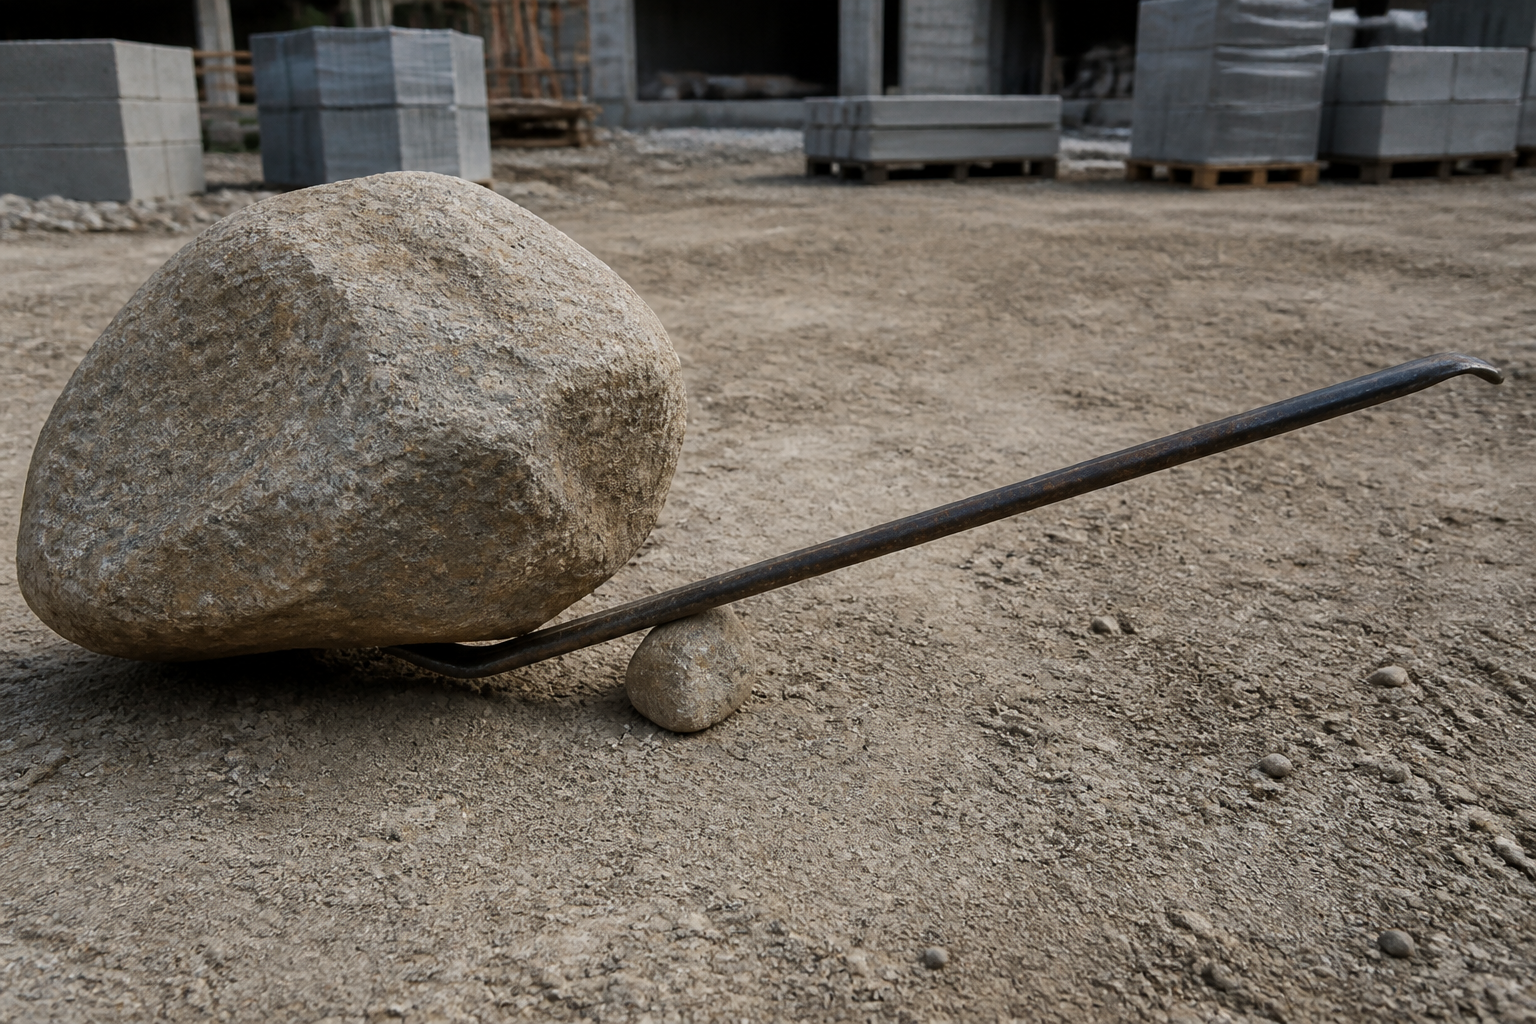
\includegraphics[width=0.55\linewidth]{images/book1/ai/g3-levers-crowbar.png}

{\small The crowbar at work: a small push far from the \omterm{def:g3:levers-and-scales:lever}{pivot} lifts a boulder no hand could move.}
\end{omfigure}

\section{The rule of the lever}

\begin{method}[The coin seesaw]\label{met:g3:levers-and-scales:coins}
Build a miniature seesaw to hunt for the rule:
\begin{enumerate}
  \item balance a ruler across a pencil at its middle mark;
  \item use identical coins as riders, placed at whole-number marks:
        ``a coin at $4$'' means four marks from the pencil;
  \item load both sides and note when the ruler balances.
\end{enumerate}
Try it: one coin at $6$ balances one coin at $6$. Two coins stacked
at $3$ balance one coin at $6$. Three coins at $2$ --- again balance
with one at $6$!
\end{method}

\begin{proposition}[The lever rule]\label{prop:g3:levers-and-scales:rule}
For each side of the \omterm{def:g3:levers-and-scales:lever}{lever}, multiply the number of coins by their
distance from the \omterm{def:g3:levers-and-scales:lever}{pivot}. The \omterm{def:g3:levers-and-scales:lever}{lever} balances exactly when the two
sides have the \emph{same product}:
\[
2 \text{ coins} \times 3 \text{ marks} = 6
\qquad\text{balances}\qquad
1 \text{ coin} \times 6 \text{ marks} = 6 .
\]
If one side's product is bigger, that side goes down.
\end{proposition}

\begin{omfigure}
\begin{tikzpicture}[scale=0.85]
  \draw[thick, fill=omExo, fill opacity=0.3]
    (5.5,0) -- (5.9,0.7) -- (5.1,0.7) -- cycle;
  \draw[very thick] (1.0,0.78) -- (10.0,0.78);
  \foreach \x in {1.75,2.5,3.25,4.0,4.75,6.25,7.0,7.75,8.5,9.25} {
    \draw (\x,0.7) -- (\x,0.86);
  }
  \draw[thick, fill=omDef, fill opacity=0.5] (3.25,1.09) circle (0.3);
  \draw[thick, fill=omDef, fill opacity=0.5] (3.25,1.69) circle (0.3);
  \node[above, font=\small] at (3.25,2.1) {$2$ coins at $3$};
  \draw[thick, fill=omThm, fill opacity=0.5] (9.25,1.09) circle (0.3);
  \node[above, font=\small] at (9.25,1.5) {$1$ coin at $6$};
  \node[below, font=\small] at (5.5,-0.25)
    {$2 \times 3 = 6$ on the left, $1 \times 6 = 6$ on the right:
     balance};
\end{tikzpicture}

{\small The \omterm{def:g3:levers-and-scales:lever}{lever} rule on a ruler: equal products, level bar.}
\end{omfigure}

\begin{example}[Using the rule]\label{ex:g3:levers-and-scales:using}
Four coins sit at mark $2$: their product is $4 \times 2 = 8$. To
balance them with coins at mark $4$, we need a product of $8$ there
too: $8 = 2 \times 4$, so two coins at $4$ do it. And could a single
coin balance the four? It would need to sit at mark $8$: $1 \times 8
= 8$. The lighter the rider, the farther out it must sit --- exactly
what Papa's seesaw taught us, now with numbers.
\end{example}

\section{The balance scale}

\begin{definition}[Balance scale]\label{def:g3:levers-and-scales:scale}
A \emph{balance scale}\index{balance scale} is a \omterm{def:g3:levers-and-scales:lever}{lever} built for
fairness: two pans hanging at \emph{exactly equal} distances from
the \omterm{def:g3:levers-and-scales:lever}{pivot}. With equal distances, the products match exactly when the
weights match --- so the scale tips toward the heavier pan, and
hangs level when the two pans hold equally heavy loads.
\end{definition}

\begin{omfigure}
\begin{tikzpicture}[scale=0.85]
  \draw[thick] (5.5,0) -- (5.5,2.6);
  \draw[thick] (4.9,0) -- (6.1,0);
  \draw[very thick] (2.5,2.6) -- (8.5,2.6);
  \fill (5.5,2.6) circle (2.4pt);
  \draw[thick] (2.5,2.6) -- (2.2,1.5) (2.5,2.6) -- (2.8,1.5);
  \draw[thick] (1.9,1.5) .. controls (2.5,1.05) .. (3.1,1.5);
  \draw[thick] (8.5,2.6) -- (8.2,1.5) (8.5,2.6) -- (8.8,1.5);
  \draw[thick] (7.9,1.5) .. controls (8.5,1.05) .. (9.1,1.5);
  \fill[omDef, opacity=0.5] (2.5,1.5) circle (0.28);
  \fill[omThm, opacity=0.5] (8.35,1.42) circle (0.22);
  \fill[omThm, opacity=0.5] (8.68,1.42) circle (0.22);
  \node[below, font=\small] at (5.5,-0.3)
    {equal arms: the scale compares the two pans fairly};
\end{tikzpicture}

{\small A \omterm{def:g3:levers-and-scales:scale}{balance scale}: a \omterm{def:g3:levers-and-scales:lever}{lever} with two pans at equal distances.
Level pans mean equally heavy loads.}
\end{omfigure}

\begin{example}[Weighing by comparing]\label{ex:g3:levers-and-scales:weighing}
For thousands of years, merchants sold flour, gold and pepper with
\omterm{def:g3:levers-and-scales:scale}{balance scales}: goods in one pan, little metal reference blocks in
the other, adding blocks until the pans hung level. The scale does
not know any numbers --- it only answers ``heavier'', ``lighter'' or
``equal''. But comparing with well-chosen blocks is all a fair
market needs --- and, as the last chapter of this part will show, it
is the road to measuring mass itself.
\end{example}

\begin{remark}[Check the empty scale]\label{rem:g3:levers-and-scales:fair}
A fair scale must hang level when \emph{empty}. If one arm is longer
or one pan heavier, the products differ before the goods even
arrive, and every weighing after that cheats. Honest merchants
proved their empty scale level in front of the customer --- an old,
wordless way of saying ``fair play''.
\end{remark}

\section{Exercises}

\begin{exercise}[$\star$]\label{exo:g3:levers-and-scales:1}
Point out the \omterm{def:g3:levers-and-scales:lever}{lever} and the \omterm{def:g3:levers-and-scales:lever}{pivot} in: a seesaw; \ a crowbar on a
log; \ scissors. (Scissors hide two \omterm{def:g3:levers-and-scales:lever}{levers} --- where do they
\omterm{def:g3:levers-and-scales:lever}{pivot}?)
\end{exercise}

\begin{exercise}[$\star$]\label{exo:g3:levers-and-scales:2}
To lift a heavy rock with a crowbar, should you press close to the
\omterm{def:g3:levers-and-scales:lever}{pivot} or far from it? Why, in one sentence?
\end{exercise}

\begin{exercise}[$\star$]\label{exo:g3:levers-and-scales:3}
On the coin seesaw, compute the product for: $3$ coins at mark $4$;
\ $2$ coins at mark $5$; \ $1$ coin at mark $6$. Which pairs of
these balance each other?
\end{exercise}

\begin{exercise}[$\star$]\label{exo:g3:levers-and-scales:4}
One coin sits at mark $8$ on the left. Where must you put $2$ coins
on the right to balance? And $4$ coins?
\end{exercise}

\begin{exercise}[$\star$]\label{exo:g3:levers-and-scales:5}
Left side: $3$ coins at mark $3$. Right side: $2$ coins at mark $4$.
Compute both products. Which side goes down?
\end{exercise}

\begin{exercise}[$\star$]\label{exo:g3:levers-and-scales:6}
Why are the two pans of a \omterm{def:g3:levers-and-scales:scale}{balance scale} hung at exactly equal
distances from the \omterm{def:g3:levers-and-scales:lever}{pivot}? What would a longer left arm do to every
weighing?
\end{exercise}

\begin{exercise}[$\star$]\label{exo:g3:levers-and-scales:7}
A \omterm{def:g3:levers-and-scales:scale}{balance scale} hangs level with a bag of marbles in one pan and $6$
identical blocks in the other. What do we learn about the bag? What
does the scale answer if we take one block away?
\end{exercise}

\begin{exercise}[$\star$]\label{exo:g3:levers-and-scales:8}
A seesaw: Tom weighs as much as $2$ sacks and sits at mark $3$; his
little sister weighs as much as $1$ sack. At which mark must she sit
to balance him?
\end{exercise}

\begin{exercise}[$\star$]\label{exo:g3:levers-and-scales:9}
The hammer's claw pulls a nail: your hand pushes the handle's end,
far from where the hammer head rests on the wood. Which is the
\omterm{def:g3:levers-and-scales:lever}{pivot}, and why does the nail --- which your fingers could never pull
--- come out?
\end{exercise}

\begin{exercise}[$\star\star$]\label{exo:g3:levers-and-scales:10}
Grandpa (heavy as $4$ sacks) wants to seesaw with little Zoe (heavy
as $1$ sack). The seesaw has marks $1$ to $8$ on each side. Find
\emph{two} different ways to seat them so the seesaw balances.
\end{exercise}

\begin{exercise}[$\star\star$]\label{exo:g3:levers-and-scales:11}
A cheating merchant secretly makes one arm of his scale a little
longer, and always puts the goods on the long-arm side. Do customers
get more goods than they pay for, or less? Explain with the \omterm{def:g3:levers-and-scales:lever}{lever}
rule --- and with \cref{rem:g3:levers-and-scales:fair}.
\end{exercise}
